\subsection{Desired System Architecture} \label{sec:desiredSystem}
The desired system architecture consists of a single cluster setup shown in \cref{fig:implementationSetup}.
\begin{figure}
    \centering
    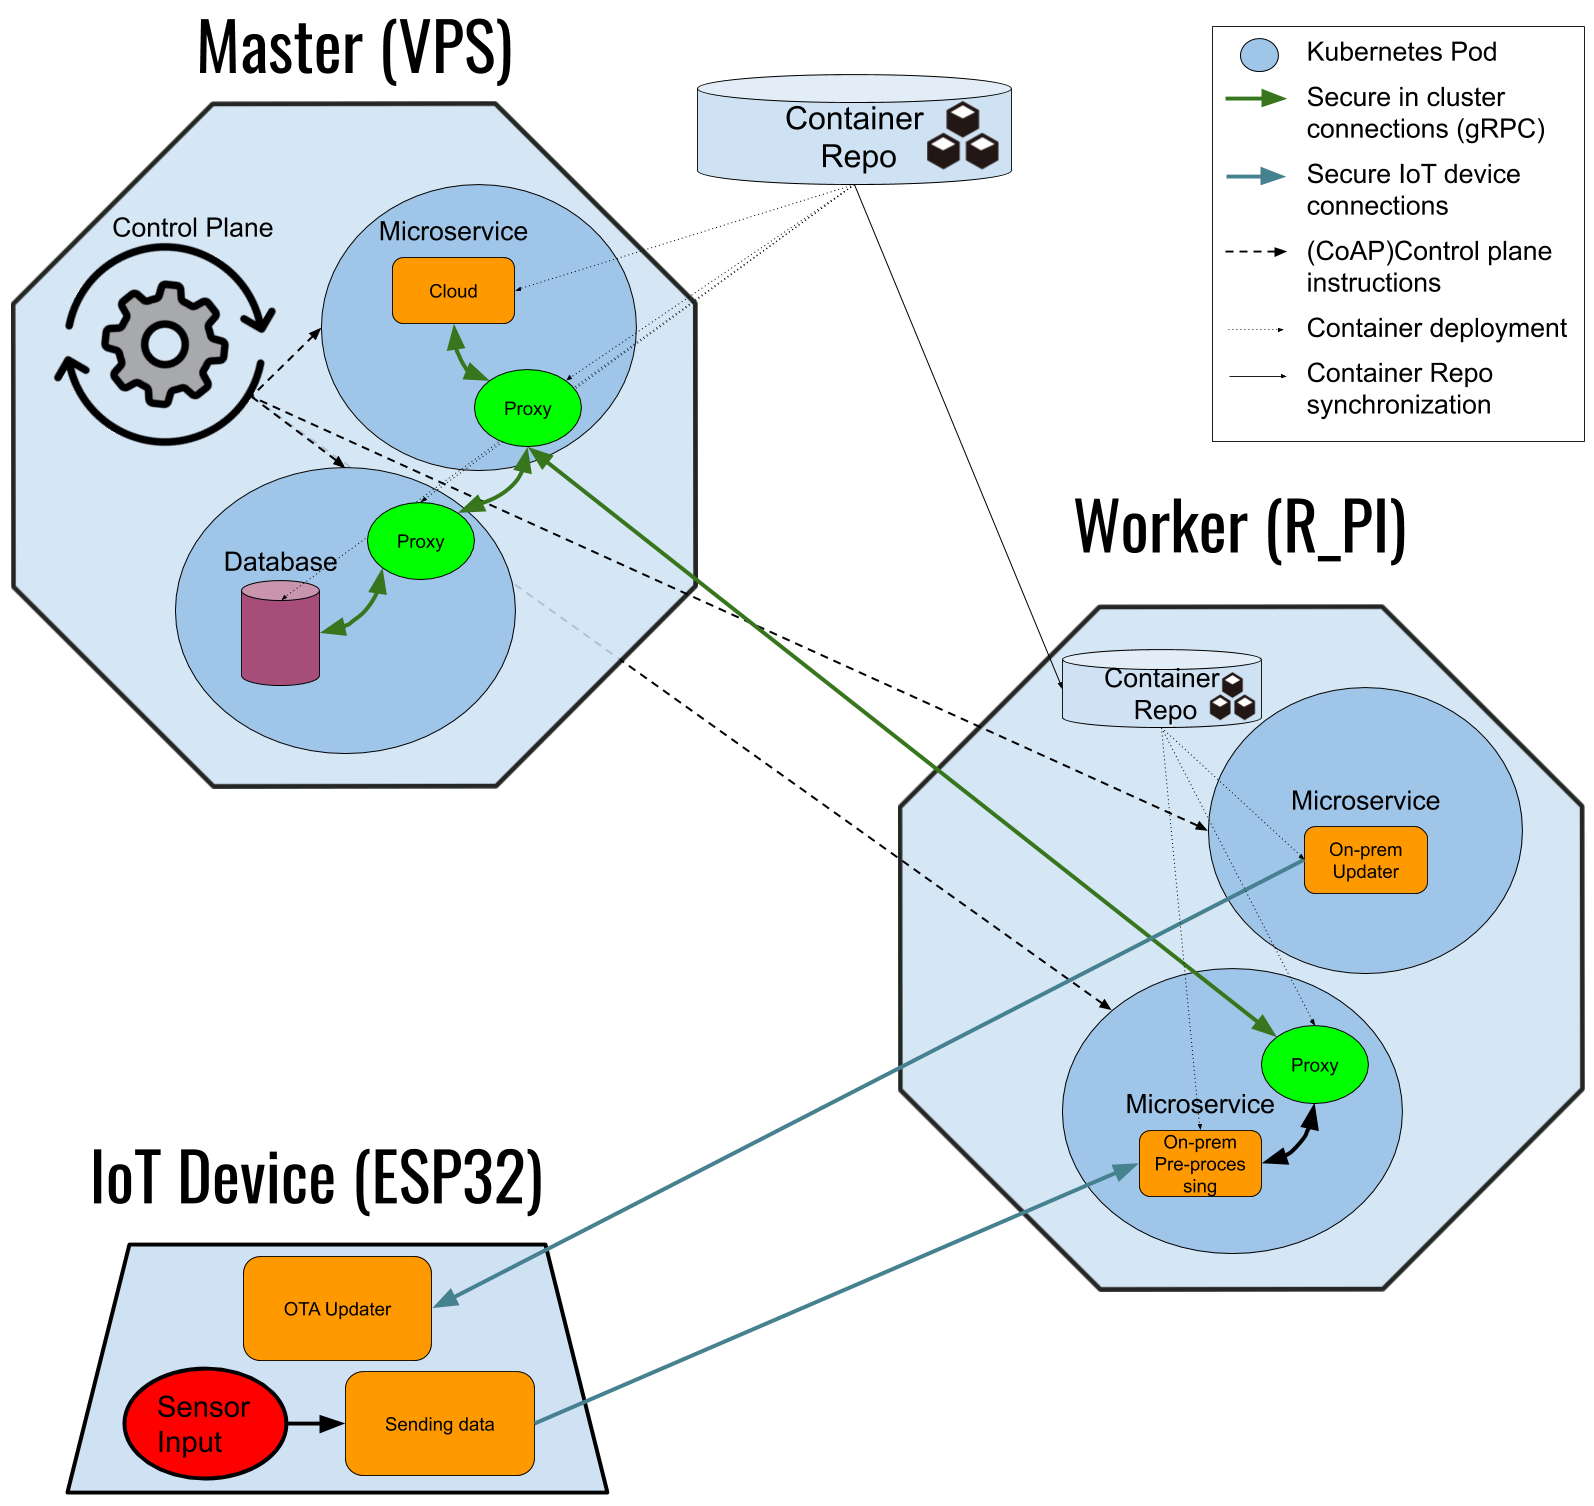
\includegraphics[scale=0.25]{figures/implementationSetup.png}
    \caption{The Desired System Architecture}
    \label{fig:implementationSetup}
\end{figure}
It has one master node running in the cloud on a VPS. This node is the primary contact point for the system administrator. The administrator defines the the desired state of the cluster and gives the specifications to the master. The master runs a control plane which works towards achieving the desired state. Here, the master runs a microservice to process the data from the IoT gateway and stores it in a distributed database. However, the database is only present on nodes which also contain the microservice, it should never be scheduled on an edge device. Istio is deployed to keep the traffic secure between the database and the microservice. It achieves this by placing a proxy container in each pod to which all traffic is redirected. It tunnels all communication inside gRPC service calls and encrypts them with mutual TLS. That is, both parties are required to show that they have a certificate from a valid certificate authority, another Istio component. So all cluster internal traffic going in and out of a pod first passes through the proxy where it is encrypted or decrypted and forwarded to the correct container inside the pod. In the figure, the proxies are the small green bubbles and the encrypted communication is shown by the green arrows.

All images for the containers are pulled from an external container repository with the ability to be mirrored. The only one doing this at the time of writing is the Docker Hub. Production images use the image digest to ensure no image manipulation and consistency between deployments. The repository for the edge relevant containers is mirrored to the edge device, a RPi. The pulling of containers is represented by the small black dotted line while the synchronization is a small black continuous line.

The RPi is fully controlled by the master node in the cloud and only schedules the pods it is supposed to schedule. It contains to services, one is for interacting with the IoT device and another one for updating the IoT device. The containers are pulled from the local container registry and only if that fails will the node contact the remote registry. 

Finally, the IoT device, an esp32, has a service listening for input from a sensor and another service listening for updates from its gateway. It connects to the gateway via WiFi and sends data via the CoAP protocol encrypted with DTLS.

This setup reflects the resource available for this thesis. The master node is running on a VPS and not bare metal, because there was no access to a bare metal server. It is a single cluster setup as the size of the project did not justify the added overhead of a multi-cluster setup.

